
\chapter{Discussion}

\section{Comparisons and Discussion of Results}\label{sec:comparaisonresults}

In this subsection, we compare the performance of different multi-robot navigation strategies.

\begin{figure}[h!]
	\begin{subfigure}[t]{0.99\linewidth}
		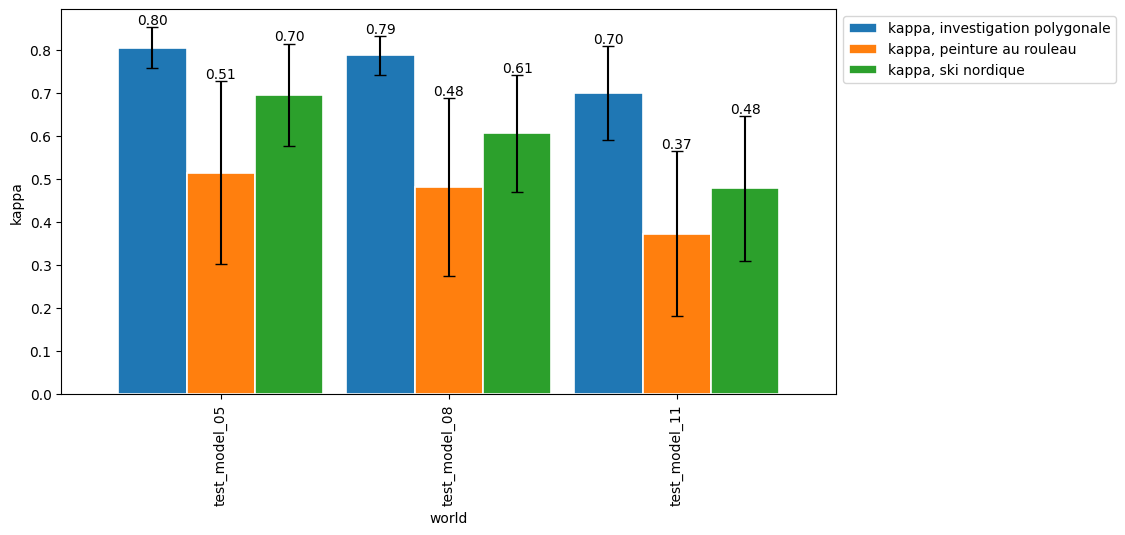
\includegraphics[width=\linewidth]{graphics/investigation_polygonale-peinture_au_rouleau_ski_nordique-kappa_for_each_world_vs_investigation_polygonale-kappa_for_each_world.png}
		\caption{$\kappa$ according to the density of the world.}
		\label{fig:investigation_polygonale-peinture_au_rouleau_ski_nordique-kappa_for_each_world_vs_investigation_polygonale-kappa_for_each_d}
	\end{subfigure}
	\hfill
	\begin{subfigure}[t]{0.99\linewidth}
		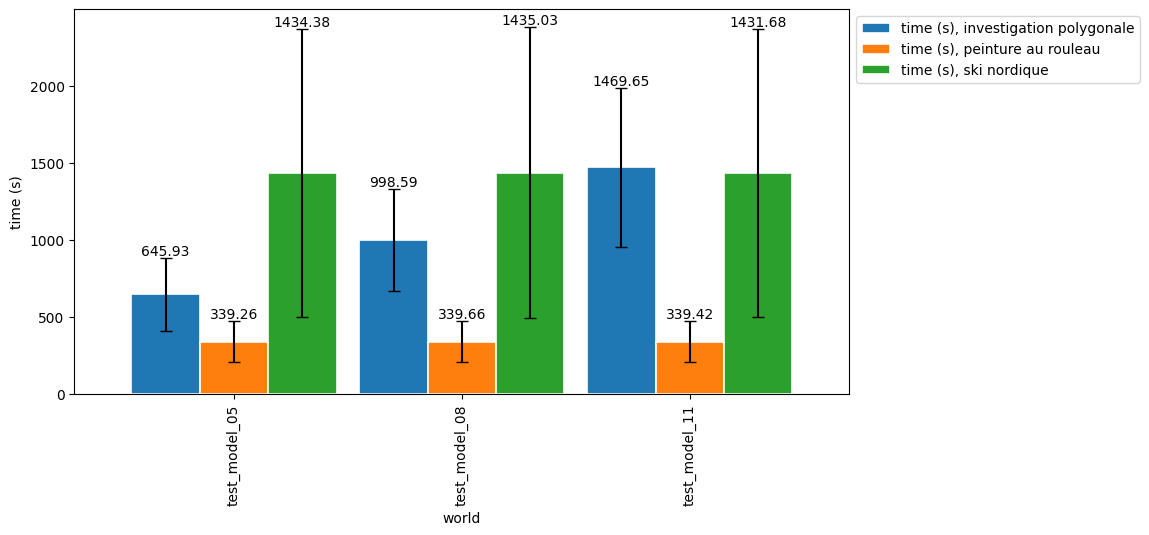
\includegraphics[width=\linewidth]{graphics/investigation_polygonale-peinture_au_rouleau_ski_nordique-time_for_each_world_vs_investigation_polygonale-time_for_each_world.png}
		\caption{Runtime based on world density.}
		\label{fig:investigation_polygonale-peinture_au_rouleau_ski_nordique-time_for_each_world_vs_investigation_polygonale-time_for_each_d}
	\end{subfigure}
	\caption{Evolution of Cohen's $\kappa$ and the execution time of the different algorithms according to the density of the world for different distances between the crawlers.}
	\label{fig:investigation_polygonale-peinture_au_rouleau_ski_nordique_for_each_world}
\end{figure}

We present on the \ref{fig:investigation_polygonale-peinture_au_rouleau_ski_nordique_for_each_world} the evolution of the Cohen score and the execution time according to the density of the world, for each algorithm.
In this figure, we have represented the scores and execution times obtained, on average, for the different values of $d$ and $s$, for the sake of readability.
We therefore obtain, on average, $d = 3$ meters and $s = 3$ meters.
A more detailed version, for each value of $d$, is available in \ref{annexe:comparaison}, in \ref{fig:investigation_polygonale-peinture_au_rouleau_ski_nordique_for_each_d}.

We can observe on the \ref{fig:investigation_polygonale-peinture_au_rouleau_ski_nordique-kappa_for_each_world_vs_investigation_polygonale-kappa_for_each_d} that the Cohen score obtained by the algorithm \textit{Polygonal Investigation} is higher than those obtained by the \textit{Roller Painting} and \textit{Nordic Skiing} algorithms.
Only the \textit{Polygonal Investigation} strategy made it possible to obtain a Cohen score considered as \textit{almost perfect agreement} (greater than 0.8) according to Landis and Koch.

We can observe on the \ref{fig:investigation_polygonale-peinture_au_rouleau_ski_nordique-time_for_each_world_vs_investigation_polygonale-time_for_each_d} that the execution time of the \textit{Roller Painting} algorithm is lower than those obtained by the \textit{Polygonal Investigation} and \textit{Nordic Skiing} algorithms.
For low map densities like those used in our experiments, the \textit{Nordic Skiing} algorithm is the slowest.
This result should be qualified.
Indeed, for higher densities, the \textit{Polygonal Investigation} algorithm becomes slower than the \textit{Nordic Skiing} algorithm, as we can already almost see for the map with 11 corrosion zones.
This is due to the fact that the \textit{Polygonal Investigation} has a linear dependence on the number of corrosion zones, while the two other algorithms do not depend on the number of corrosion zones.

\begin{table}[h!]
	\centering
	\begin{tabular}{|c|c|c|}
		\hline
		& \multicolumn{2}{c|}{\textbf{Gain in performance \textit{Polygonal Investigation}}} \\
		\hline
		\textbf{compared to} & \textbf{Cohen's $\kappa$} & \textbf{Runtime} \\
		\hline
		\textit{roll paint} & +68.39\% & +305.80\% \\
		\hline
		\textit{Nordic skiing} & +27.92\% & -3.92\% \\
		\hline
	\end{tabular}
	\caption{Performance gain provided by the \textit{Polygonal Investigation} strategy compared to the \textit{Roller Painting} and \textit{Nordic Skiing} strategies.}
	\label{tab:gain}
\end{table}

The \ref{tab:gain} presents the performance gain provided by the \textit{Polygonal Investigation} strategy compared to the \textit{Roller Painting} and \textit{Nordic Skiing} strategies.
Here, we considered the investigation time of the \textit{Polygonal Investigation} strategy to be equal to the sum of the investigation times of the \textit{Polygonal Investigation} strategy and the \textit{Roller Painting} strategy since the first strategy is based on the second to explore the corrosion zones.
We can observe that the \textit{Polygonal Investigation} algorithm achieves a Cohen score 68.39\% higher than that obtained by the \textit{Roller Painting} algorithm, although it is much slower than this last.
On the other hand, the \textit{Polygonal Investigation} algorithm makes it possible to obtain a Cohen score 27.92\% higher than that obtained by the algorithm \textit{Nordic Skiing}, while being faster than the latter.

The \textit{Polygonal Investigation} strategy is therefore the best strategy in terms of performance, in our experiments, as well as a trade-off between the Cohen score and the execution time.
The performance gain provided by the \textit{Polygonal Investigation} strategy  is explained by the fact that this strategy permits to greatly vary the vector of the signal emitted and received by the robots, and therefore to approach the convex envelope of the corrosion zones as closely as possible.


\section{Theoretical Study of Properties of the Solution Proposal}

\subsection*{\textit{Nordic Skiing} Navigation Strategy}

\begin{proposition}
	The angle of the signal emitted and received by the robots, for the \textit{Nordic Skiing} navigation strategy, varies between $-\tan^{-1}(\frac{s}{d})$ and $\tan ^{-1}(\frac{s}{d})$.
	\label{prop:angle_ski_nordique}
\end{proposition}

We can observe the result of the \ref{prop:angle_ski_nordique}, relying on the properties of trigonometry and the definition of the tangent function.
We explain in \ref{fig:angle_ski_nordique} the process undertaken to find $\alpha = -\tan^{-1}(\frac{s}{d})$.
This proposal allows us to quantify the range of the orientation of the signal emitted and received by the robots.

\begin{figure}[h!]
	\centering
	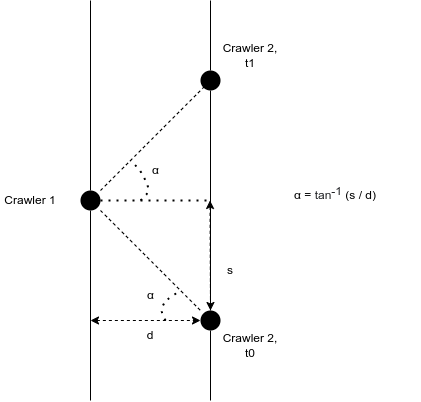
\includegraphics[scale=0.9]{graphics/angle_ski_nordique.png}
	\caption{Orientation of the transmitted and received signal for the \textit{Nordic Skiing} navigation strategy.}
	\label{fig:angle_ski_nordique}
\end{figure}

\subsection*{\textit{Polygonal Investigation} Navigation Strategy}

\begin{proposition}[Completeness]
	The \textit{Polygonal Investigation} navigation strategy, defined by a polygon, $P$ allows to cover all points inside the polygon $P$.
	\label{prop:completeness}
\end{proposition}
\begin{proof}
	Let's prove \ref{prop:completeness}.
	\begin{itemize}
		\item Let $P$ be a convex polygon with $p$ vertices used for the \textit{Polygonal Investigation} navigation strategy.
		\item For simplicity, we consider a strategy with 2 robots, but the proof remains similarly the same for $n > 2$ robots.
		\item Consider the robot $r_1$ at vertex $s_1$ of polygon $P$ and the robot $r_2$ at vertex $s_2$ of polygon $P$.
		\item Let $p$ be a point inside the polygon $P$.
		\item Then, there exists a point $p'$ such that $p$ is on the segment $[s_1, p']$ and $p'$ is on the edge of the polygon $P$, by definition of the convexity of $P$.
		\item By definition of the \textit{Polygonal Investigation} navigation strategy, the robot $r_2$ moves on the contours of the polygon $P$ and therefore in particular on the point $p'$.
		\item We therefore have for any point $p$ inside the polygon $P$, there is a pair of positions for the robots $r_1$ and $r_2$ such that $p$ is on the segment formed by the points where robots $r_1$ and $r_2$ are located.
		\item So all points inside the polygon $P$ are covered by the \textit{Polygonal Investigation} navigation strategy.
	\end{itemize}
\end{proof}

\begin{proposition}
	The approximation of the convex envelope of the corrosion zones at the end of the Polygonal Investigation, with a polygon with $p$ vertices, $p \in \mathbb{N}$, is a polygon of at most $2 p$ vertices.
	\label{prop:poly_dimensions}
\end{proposition}
\begin{proof}
	Let us give an intuition of the proof of the \ref{prop:poly_dimensions}.
	\begin{itemize}
		\item We have, for each vertex of the polygon, there are two straight lines passing through this point and touching the corrosion zone without crossing it.
		\item We therefore have, for a vertex of the polygon, at most two lines which participate in the construction of the approximation of the convex envelope and therefore, of which a segment of these lines is an edge of the approximation of the convex envelope.
		\item We therefore have, for a vertex of the polygon, at most two edges of the approximation of the convex envelope.
		\item We therefore have, for a polygon with $p$ vertices, at most $2p$ edges of the convex envelope approximation.
		\item We therefore have, for a polygon with $p$ vertices, at most $2p$ vertices of the convex envelope approximation.
	\end{itemize}
\end{proof}

\begin{conjecture}
	If the number of vertices $p$ of the polygon $P$, used during the \textit{Polygonal Investigation} algorithm, tends towards infinity, and therefore approximate a circle, then the approximation of the convex envelope of the corrosion zone at the end of the \textit{Polygonal Investigation} strategy is the convex envelope itself.
	\label{prop:circle}
\end{conjecture}

